\label{sec:5.4}

%%%%%%%%%%%%%%%%%%%%%%%%%%%%%%%%%%%%%%%%%%%%%%%%%%%%%%%
%(Prakash) Discuss SHA/MUX linearity
%%%%%%%%%%%%%%%%%%%%%%%%%%%%%%%%%%%%%%%%%%%%%%%%%%%%%%%

The input signals are sampled at a rate of 2 MS/s, multiplexed by 8 and digitized by one of two calibrated 12-bit pipelined ADCs operating at 16 MS/s. The linearity of the ADC to a small extent depends on the linearity of the SHA/MUX circuit aswell. 
The ability to configure and isolate the MUX's turned out to be very helpful to debug the SHA/MUX linearity issue. The linearity of the ADC is approximately reduced by 0.3 LSB when SHA is in free running mode, i.e. MUX is operating. 

%Studies were performed at two configuration settings, forzen SHA mode and free running SHA mode. Nominal operation is free running SHA mode. 

During the Frozen SHA mode, the ADC will oversample the SHA output by a factor of 8 and the linearity of the ADC can be calculated by taking any of the samples. We observed that the overall linearity was different for different sample sets. Figure \ref{fig:sha_sample_hist} shows ADC sampling with frozen SHA.
\begin{figure}[h!]
\centering
  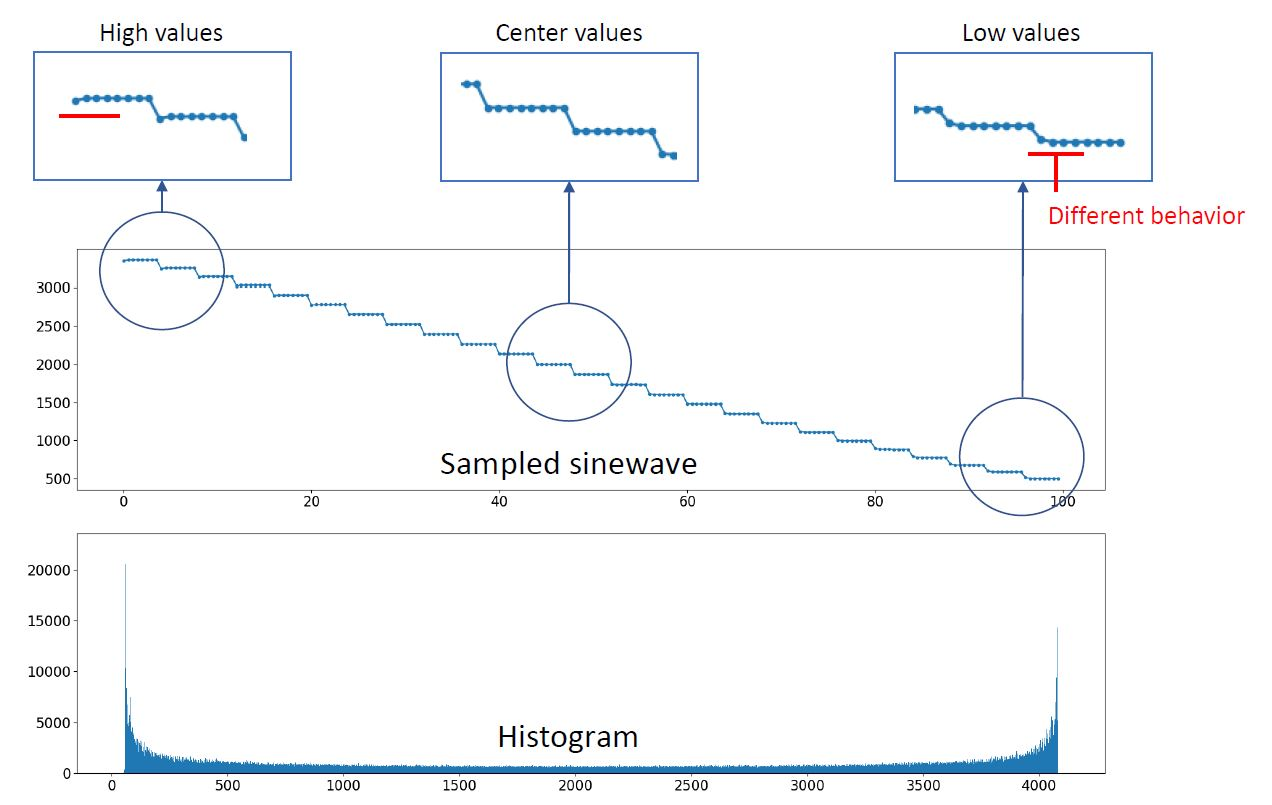
\includegraphics[width=0.7\linewidth]{figures/prakash_fig/sha_sample_hist.JPG}
  \caption{Histogram of ADC sampling in frozen SHA configuration}
  \label{fig:sha_sample_hist}
\end{figure}
The non-linearity could be affected by SHA or MUX or a combination of both. To verify if the SHA op-amps are causing any non-linearity. Figure~\ref{fig:linearity_sha_current} shows the linearity of ADC measured by looking at the second sample of channel 7 at 40$\mu$A, 50$\mu$A (default) and 60$\mu$A bias currents. 
\begin{figure}[h!]
\centering
  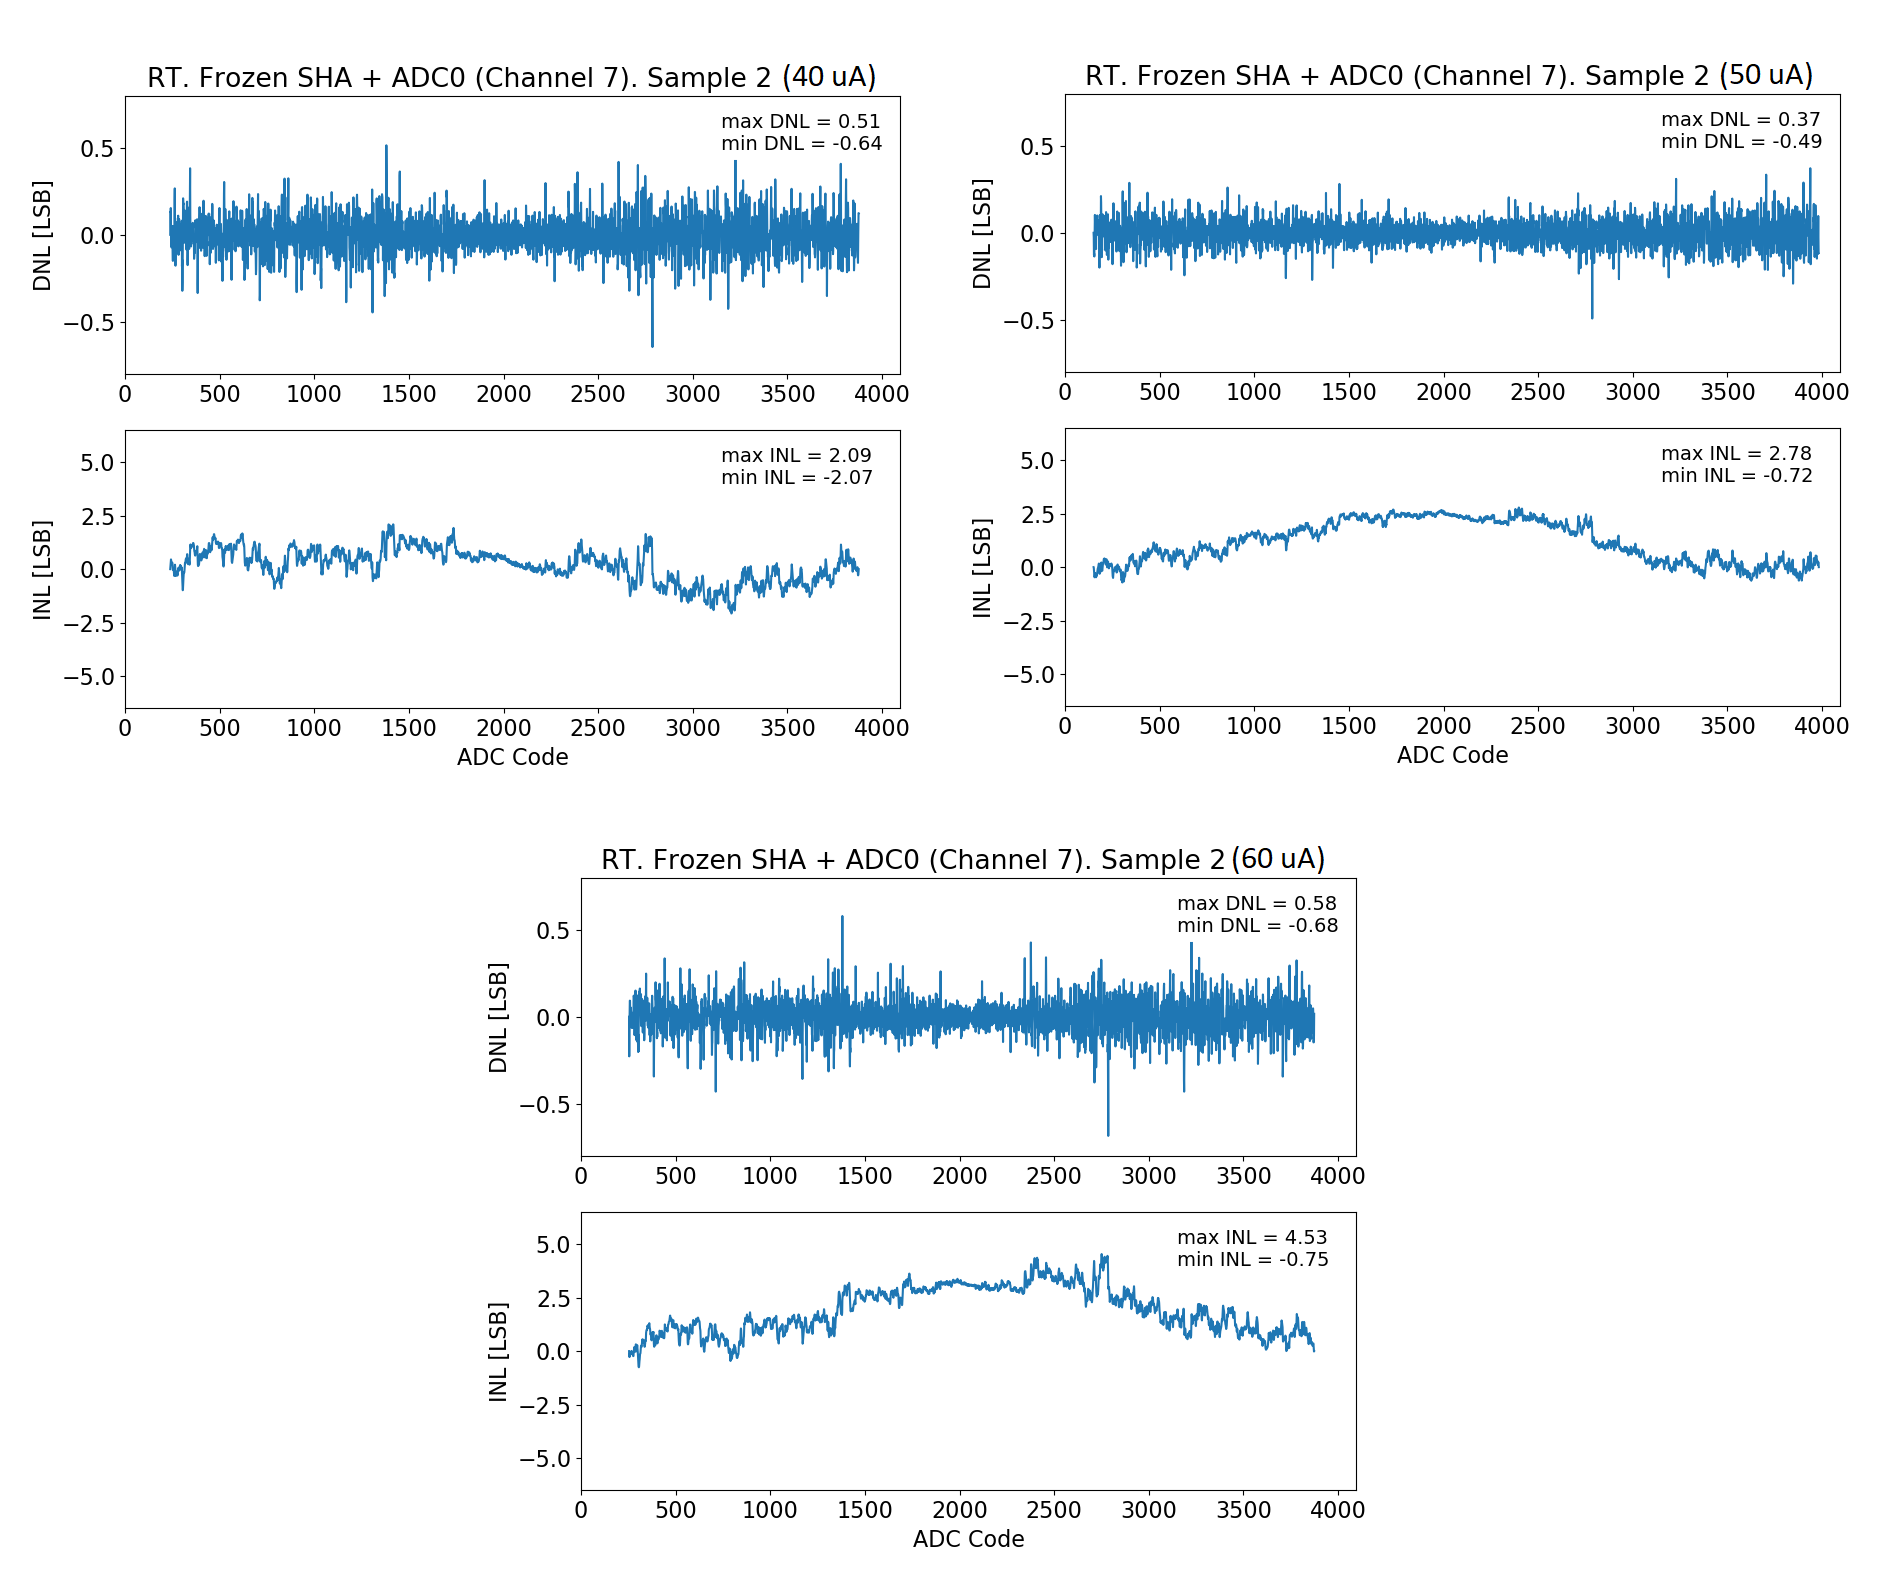
\includegraphics[width=1.0\linewidth]{figures/prakash_fig/linearity_sha_current.png}
  \caption{Linearity of ADC at room temperature with SHA bias current configured to 40, 50, and 60 $\mu$A.}
  \label{fig:linearity_sha_current}
\end{figure}
Varying the SHA bias currents did not affect the overall linearity of the ADC. To verify if the MUX's were causing the non-linearity, we reduced the sampling speed. Figure~\ref{fig:linearity_mux_speed} shows the linearity at different sampling clocks. 
\begin{figure}[h!]
\centering
  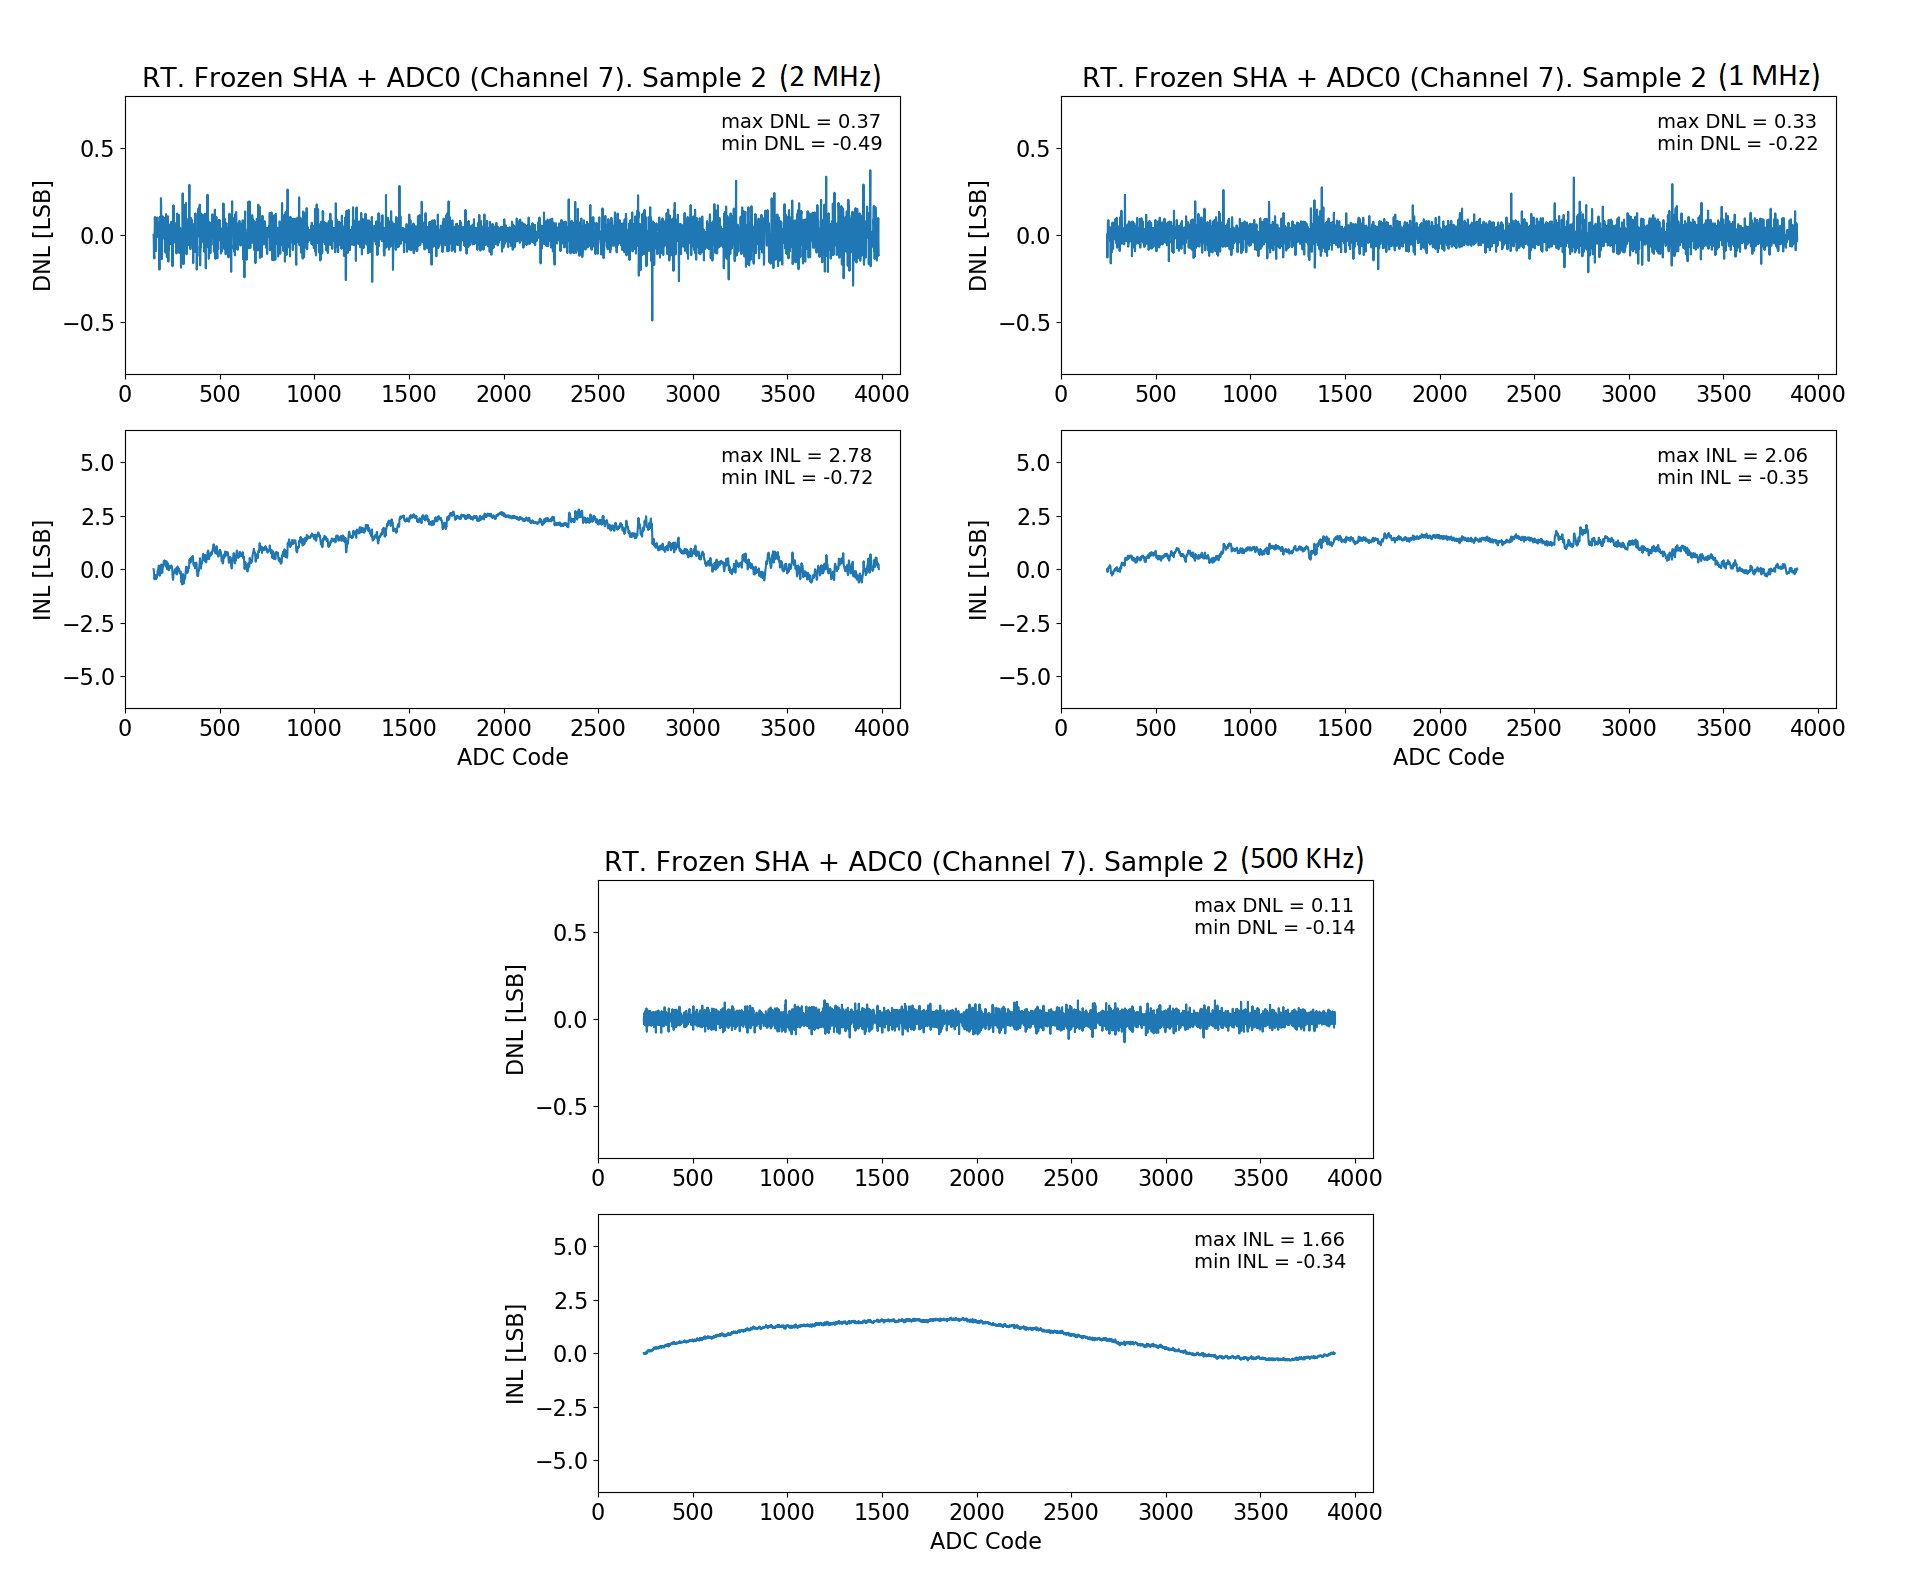
\includegraphics[width=1.0\linewidth]{figures/prakash_fig/linearity_mux_speed.png}
  \caption{Linearity of ADC at room temperature with 2, 1, 0.5 MHz sampling frequencies.}
  \label{fig:linearity_mux_speed}
\end{figure}

Reducing the sampling frequency improves the linearity significantly. The MUX's seem to be causing the non-linearity and we believe the kickback is the main source of the problem. To address this problem we plan to redesign the MUX to be much faster.

We also observed spikes in the DNL plots while the ColdADC was configured to free running SHA mode. These spikes however reduced when he ColdADC was configured to frozen SHA mode. Figures \ref{fig:linearity_freesha} and \ref{fig:linearity_frozensha} show the difference in linearity for free running and frozen SHA. These measurements were performed with nominal clocks and nominal reference voltages.  
\begin{figure}[h!]
\centering
  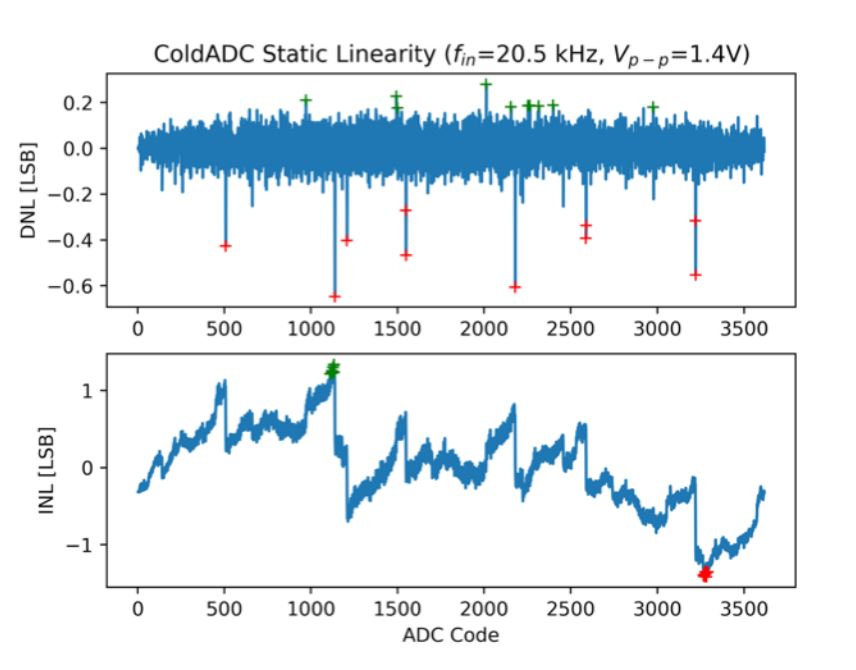
\includegraphics[width=0.7\linewidth]{figures/prakash_fig/linearity_freesha.JPG}
  \caption[Linearity of the ADC with single ended input with free running SHA]{Linearity of the ADC with single ended input with free running SHA: These measurements were taken at LN2 temperature. During the free running SHA configuration, the MUX's introduces additional spikes in the DNL}
  \label{fig:linearity_freesha}
\end{figure}
\begin{figure}[h!]
\centering
  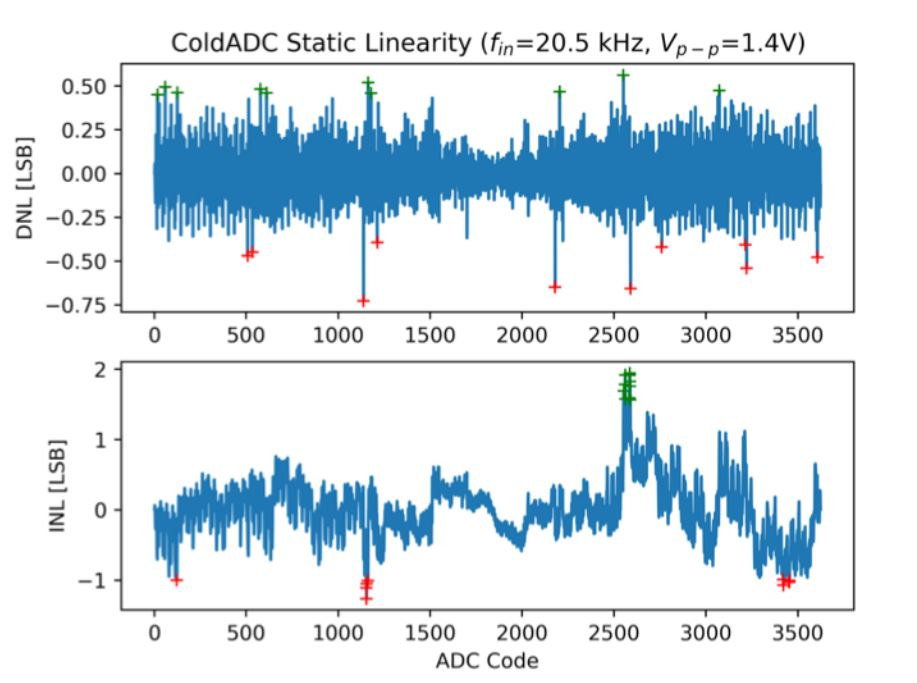
\includegraphics[width=0.7\linewidth]{figures/prakash_fig/linearity_frozensha.JPG}
  \caption[Linearity of the ADC with single ended input with frozen SHA]{Linearity of the ADC with single ended input with frozen SHA: These measurements were taken at LN2 temperature}
  \label{fig:linearity_frozensha}
\end{figure}

Another observation was that the DNL spikes were larger when the ASIC was cooled down, a possible explanation for this is the ON resistance of the switches (MUX) is significantly larger at cold than in warm. Redesigning the MUX to be faster will solve this problem aswell.  

Evidence of linearity degradation only during the free running SHA mode indicate couple other possible issues: possible overlapping of the clocks for the MUX's and/or insufficient settling of MUX's. It is very difficult to simulate MUX's effects on ADC linearity. We are still in the process of understanding and proving the root cause for linearity degradation in simulations. To fix this, we will redesign the MUX's to be faster and improve the clocking scheme. 


